%==============================================================================
% experimental-setup.tex
%==============================================================================

\part{Appendices}
\label{part:appendices}

\chapter{Experimental Setup}
\label{chap:experimental-setup}

The performance results were obtained on the following two machines.

\section{Intel Core2 Duo}
\label{sec:experimental-setup-marvin}

TODO: Describe marvin

See Figure \ref{fig:experimental-setup-marvin}.

\begin{figure}[htb]
  \centering
  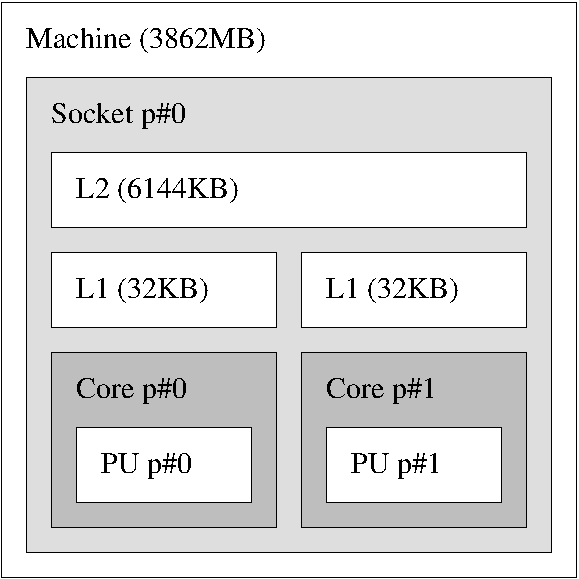
\includegraphics[width=0.5\textwidth]{experimental-setup/marvin}
  \caption[Intel Core2 Duo]{Intel Core2 Duo}
  \label{fig:experimental-setup-marvin}
\end{figure}

\section{Intel Nehalem}
\label{sec:experimental-setup-mafushi}

This system includes two Intel Xeon E5520 quad-core processors based
on the Intel Nehalem microarchitecture. The machine has 12 GB RAM;
each processor has a direct connection to half of the memory space via
an integrated memory controller (see Figure
\ref{fig:experimental-setup-mafushi}). The on-chip integrated memory
controller (IMC) provides a maximum theoretical throughput of 26 GB/s.

In addition, each processor has two QuickPath Interconnect (QPI)
interfaces \cite{R.A.MaddoxG.Singh2009}, one connecting to the remote
processor and one to the I/O hub. The interconnect has a theoretical
maximum throughput of 11.72 GB/s in one direction and 23.44 GB/s in
both directions.

% TODO: Fix reference

Each core has its separate level 1 and level 2 caches, but the
per-processor 8 MB level 3 cache is shared between all cores of the
same processor. The Intel documentation considers the level 3 cache
and the memory controllers of a processor as a separate subsystem and
refers to this subsystem as the uncore. 

We sometimes refer to a processor as a node to emphasize its
participation in forming a (large-scale) parallel system.

\begin{figure}[htb]
  \centering
  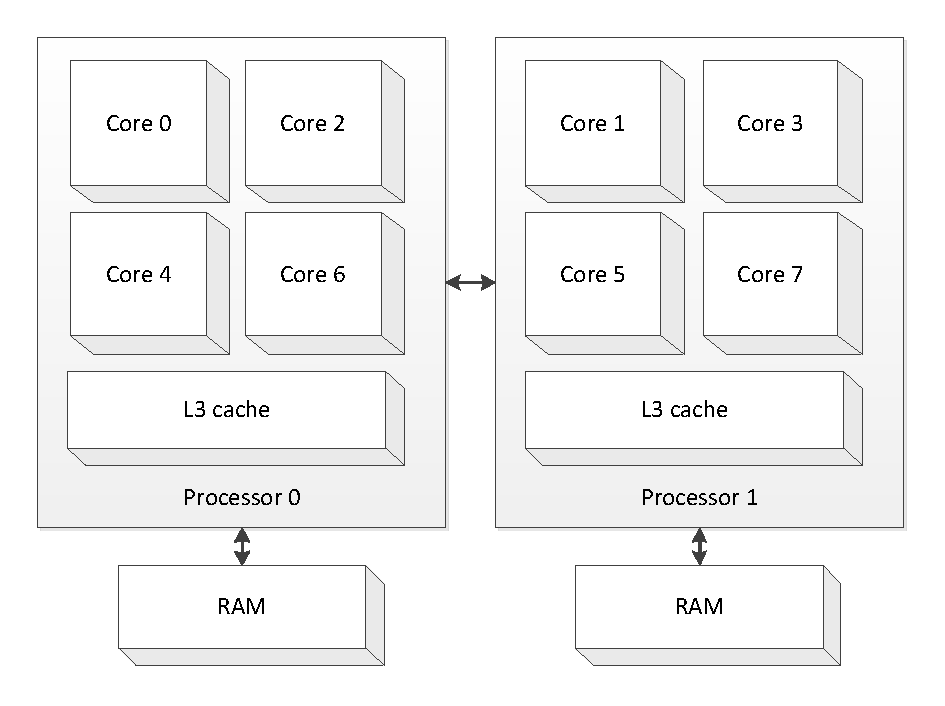
\includegraphics[width=0.8\textwidth]{experimental-setup/mafushi}
  \caption[Intel Nehalem in a two-processor configuration]{Intel
    Nehalem in a two-processor configuration}
  \label{fig:experimental-setup-mafushi}
\end{figure}


%%% Local Variables: 
%%% mode: latex
%%% TeX-master: "thesis"
%%% End: 
